%Start
%
%
%******************************************************************************************************%
%                                  linear harmonic oscillator                                          %
%******************************************************************************************************%								 
% Version 1,                                                                                           %
% 09.07.2023                                                                                           %
% L.Lentz@umwelt-campus.de                                                                             %
%******************************************************************************************************%
%
%
\documentclass[tikz,border=10pt]{standalone}
\usetikzlibrary{calc,intersections,backgrounds}
\usepackage{ifthen}
%
\tikzset{
axes/.style = {line width = 0.7pt},
grid/.style = {line width = 0.3pt,color = gray},
plots/.style = {samples=300,smooth,line width = 0.7pt}
}
%
\begin{document}
%
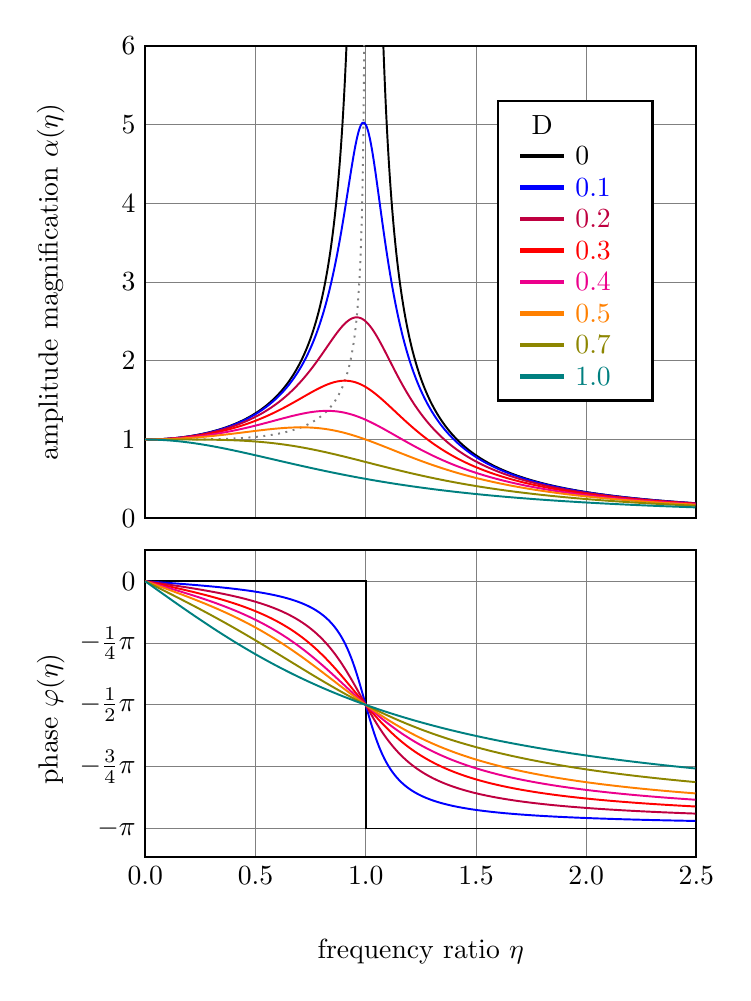
\begin{tikzpicture}
%
\def\width{7}
%
\def\Dlist{0,0.1,0.2,0.3,0.4,0.5,0.7,1.0}
\def\colorlist{{"black","blue","purple","red","magenta","orange","olive","teal"}}
\def\xlist{0.0,0.5,1.0,1.5,2.0,2.5}
\def\ampylist{0,1,2,3,4,5,6}
\def\phaseylist{0/0,-0.25*3.14/$-\frac{1}{4}\pi$,-0.5*3.14/$-\frac{1}{2}\pi$,-0.75*3.14/$-\frac{3}{4}\pi$,-3.14/$-\pi$}
%
\def\xmax{2.5}
\def\ymax{6}
\def\ymin{-3.5}
\def\pos{0.8cm}
\def\tagshift{1.2cm}
%
% scale x-axis to match width
\pgfmathsetmacro{\xsc}{\width/\xmax}
\begin{scope}[xscale=\xsc]
	%
	% x-grid and x-tick-labels
	\foreach \x in \xlist {
		\draw[grid](\x,0)--(\x,\ymax);
		\draw[grid,yshift=-\pos](\x,\pos/2)--(\x,\ymin);
		\node[yshift=-\pos, anchor = north] at (\x,\ymin){\x};
	}
	%
	% y-grid and y-tick-labels
	\foreach \y in \ampylist{
		\draw[grid](0,\y)--(\xmax,\y)node[at start, left, color = black]{\y};
	}
	\foreach \y/\tag in \phaseylist{
		\draw[grid,yshift=-\pos](0,\y)--(\xmax,\y)node[at start, left, color = black]{\tag};
	}
	%
	% Frames
	\draw[axes](0,0)rectangle(\xmax,\ymax);
	\draw[axes,yshift=-\pos] (0,\pos/2)rectangle(\xmax,\ymin);
	%
	% Legend box
	\draw[fill=white,draw=black,line width=1pt] (1.6,5.3) rectangle (2.3,1.5);
	\node[] at (1.8,5){D};
	%
	%plot curves for D-values from list
	\foreach \D [count=\i] in \Dlist {
	%
		\pgfmathsetmacro{\c}{\colorlist[\i-1]} % get color 
		\draw[line width = 1.5pt,color=\c] (1.7,5-\i*0.4)--(1.9,5-\i*0.4)node[at end,right]{\D}; % legend entry
		%
		\begin{scope}
			\clip[](0,0) rectangle (\xmax,\ymax);% clip plot to frame
			\ifthenelse{\i=1}
   				{
   				\draw[domain=0.01:0.707,variable=\x,plots,color=gray,dotted] plot ({sqrt(1-2*\x^2)},{1/2*sqrt(1/(\x^2-\x^4))});
       				};
			\ifthenelse{\lengthtest{\D pt = 0pt}}
				{
				\draw[domain=0:0.99,variable=\x,plots,color=\c] plot (\x,{sqrt(1/((2*\D*\x)^2+(1-\x^2)^2))});
				\draw[domain=1.01:\xmax,variable=\x,plots,color=\c] plot (\x,{sqrt(1/((2*\D*\x)^2+(1-\x^2)^2))});
				}
				{
				\draw[domain=0:\xmax,variable=\x,plots,color=\c] plot (\x,{sqrt(1/((2*\D*\x)^2+(1-\x^2)^2))});% plot amplitude magnification
				};
		\end{scope}
		%
		\ifthenelse{\lengthtest{\D pt = 0pt}}
			{
			\draw[yshift=-\pos,line width = 0.7pt,color=\c] plot coordinates {(0,0)  (1,0) (1,-3.14) (\xmax, -3.14)};
			}
			{
			\draw[yshift=-\pos,domain=0:\xmax,variable=\x,plots,color=\c] plot (\x,{3.14/180*atan2(-2*\D*\x,1-\x^2)});% plot phase
			};
	%
	}
	% axis labels
	\node[rotate=90] at($(0,\ymax/2)+(-\tagshift/\xsc,0)$){amplitude magnification $\alpha(\eta)$};
	\node[yshift = -\pos,rotate=90] at($(0,\ymin/2)+(-\tagshift/\xsc,0)$){phase $\varphi(\eta)$};
	\node[yshift = -\pos] at($(\xmax/2,\ymin)+(0,-\tagshift)$){frequency ratio $\eta$};
	%
\end{scope}
%
\end{tikzpicture}
%
\end{document}
%
%
%Ende
